% Les maths d'un nœud TikZ restent des maths : `~:~` n'y est pas signalé.
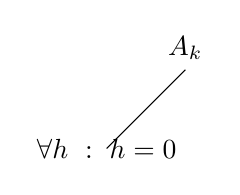
\begin{tikzpicture}
  \node at (0, 0) {$\forall h ~:~ h = 0$};
  \draw (0, 0) -- (1, 1) node[above] {$A_k$};
\end{tikzpicture}
Tout sous espace fermé est complet. % attendu: C4
